
\documentclass[english,hyperref={pdftex,pdfpagemode=UseNone,hidelinks}]{tufte-handout}
\usepackage[T1]{fontenc}
\usepackage[latin9]{inputenc}
\usepackage{amsmath}
\usepackage{math}
\usepackage{mathtools}
\usepackage{hyperref}
\hypersetup{
    colorlinks=magenta,
    linkcolor=magenta,
    filecolor=magenta,      
    urlcolor=magenta,
    }
\makeatletter




\title{Problem Set 1}

\author{Quantitative Economics, Fall 2024}


\makeatother

\usepackage{babel}
\begin{document}
\maketitle
This problem set consists of six problems. You have XXX weeks to solve them and submit your solutions (XXX 11:59 PM). You can work in teams of up to three students.   

$$v(X,D) = \max_F  p \cdot \min \left\{D,X\right\} - c \cdot F - K \cdot \mathbb{I}_{F>0}  +  \beta E_{X,D} v(\min\left\{\max \left\{X-D,0\right\} + F,\bar{X}\right\},D^\prime)$$ 


\subsection*{Problem 1: A simple differential equation}
We have 
\begin{align*}
    \frac{dy}{dx} = y\of{x},
\end{align*}
with the initial condition $y(0) = 1$. Our task to find $\of{x}$ that satisfies the above. It is straightforward to show that it must be $y\of{x}=\exp{x}$.\footnote{Just differentiate $\exp{x}$ to verify it is true.} 
Your task is to write a function that takes the step size $h$ as an argument and returns the value of $y$ at $x = 1$. 

\subsection*{Problem 1: Solow model}

Recall the law of motion for capital in the Solow model: 
\begin{align*}
    K_{t+1} = sY_t + (1-\delta)K_t,
\end{align*} where $K_t$ is the capital stock, $Y_t$ is the output, $s\in\bp{0,1}$ is the saving rate, and $\delta$ is the depreciation rate. The output is given by the Cobb-Douglas production function: 
\begin{align*}
    Y_t = K_t^\alpha \bp{A_t N_t}^{1-\alpha},
\end{align*}
where $A_t$ is the total factor productivity, $N_t$ is the labor force, and $\alpha\in\bp{0,1}$ is the output elasticity with respect to capital. In addition $g$ is the growth rate of TFP and $n$ is the growth rate of the labor force.\footnote{This means that $A_{t+1} = g A_t$ and $N_{t+1} = n N_t$.}

Recall that capital per unit of effective labor, $k_t \equiv \frac{K_t}{A_t N_t }$ follows\footnote{Use $K_{t+t} = s K_t^\a \bp{A_t N_t}^{1-\a} + (1-\delta)K_t$. Divide it by $A_t N_t$ and use the definition of $k_t$ together with $A_{t+1} = g A_t$ and $N_{t+1} = n N_t$ to get the formula.} \begin{align*}
    n g k_{t+1} = s k_t^\a + (1-\delta)k_t.
\end{align*}
The balance growth path level of capital per unit of effective labor is given by
\begin{align*}
    k = \bp{\frac{s}{\delta+ng-1}}^{1/(1-\alpha)}
\end{align*}

Your task is to write a script that illustrates the workings of the Solow model: it is a collection of simple exercises, that one could easily solve using a spreadsheet. Try to recycle functions that you design for one exercise in the next ones: in particular, try to write a function that calculate the capital per unit of effective labor in any period $t$ given the parameters of the model and the initial capital per unit of effective labor. Resist temptation to hard-code parameter values.  

\begin{enumerate}
    \item We will study how the speed of convergence to the balanced growth path depends on the parameters of the model. Suppose that the initial capital per effective labor is $k_0 = \rho k$, with $\rho \in \bp{0,1}$. After how many periods the gap between $k_t$ and $k$ (relative to $k$) will be smaller than half of the initial gap? Your code should take the four parameters of the model: $\a,\d,g,n$ and $\rho$ as inputs and return the smallest integer number of periods that satisfies the condition above as an output. 
    What is this number for $\a = 0.3,\d = 0.1,g = 1.01, n = 1.005$, and $\rho = 0.75$? Does it increase or decrease if we increase $\a,\d,g,n$ by $1\%$ (each separately)? 

    \item Assume there are two economies that are identical except for $\rho$. We have $\rho_1<\rho_2$, so the second economy starts closer to the balanced growth path. Write a function that takes the four parameters of the model and $\rho_1$ and $\rho_2$ as inputs and returns the number of periods after which the ratio of capital per effective labor in the first economy to the second economy will be smaller than half of the initial gap. What is this number for $\a = 0.3,\d = 0.1,g = 1.01, n = 1.005$, and $\rho_1 = 0.25, \rho_2 = 0.50$? Does it increase or decrease if we increase $\a,\d,g,n$ by $1\%$ (each separately)? 

    \item Write a function that creates the following plot. On the horizontal axis we will have the number of periods: $t=0,1,\ldots$. We will plot the natural logarithm of output in the economy, $\ln\of{Y_t}$\footnote{We have $Y_t = k_t^\a A_t N_t$}  (solid line). Normalize $A_0,N_0=1$. In addition, we will plot the natural logarithm of output on the balanced growth path (dotted line).\footnote{It is given by $Y_t = k^\a A_t N_t$.}  You function should take the four parameters of the model, $\rho$, and the number of periods $T$ as inputs and return the plot. Make sure that the plot is well-labeled and has a legend.
\end{enumerate}



\subsection*{Problem 2: Julia basics and Random.jl}

Recall the Lindeberg-Levy Central Limit Theorem:\footnote{See \href{https://en.wikipedia.org/wiki/Central_limit_theorem}{here} for more details.} 
\begin{align*}
    \frac{\bar X_n - \mu}{\sigma\sqrt{n}} \xrightarrow{d} N(0, 1)
\end{align*}
for $\bc{X_1,X_2,\ldots}$ i.i.d. with $E\bs{X_i} = \mu$ and $Var\bs{X_i} = \sigma^2<\infty$. Here $\bar X_n = \frac{1}{n}\sum_{i=1}^n X_i$.

Your task is to illustrate it for $X_i \sim \text{Pois}\of{\lambda}$.\footnote{Recall that for $X \sim \text{Pois}\of{\lambda}$, $E\bs{X} = \lambda$ and $Var\bs{X} = \lambda$.} 
You will have to plot four histograms of 1000 realizations of $\bar X_n$, for $n = 5, 25, 100, 1000$, (in blue) and superimpose the density of $N(0,1)$ on each of them (in red). \begin{marginfigure}
    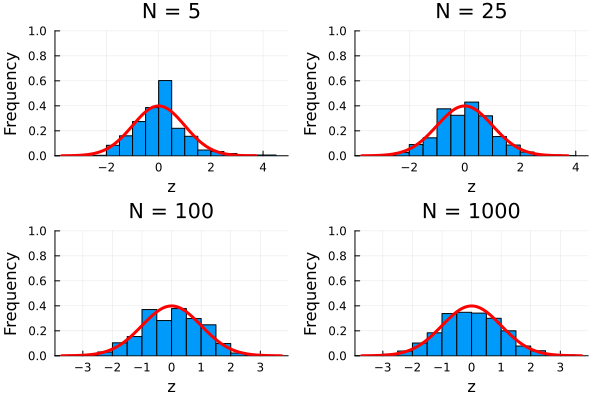
\includegraphics[width=1\textwidth]{clt.png}
    \caption{You should produce something like this.}
\end{marginfigure}

We will set $\lambda = 1$ for simplicity. Your task is to write code that will generate the requested plots. There is more than one solution! For example: you can calculate averages by summation or by using a function that already exists in Julia.\footnote{I do not ask you to write first a function that works for arbitrary argument values (including even the density function). I however encourage you to think how to make your code well-organized, easy to read and modular. Use this simple exercise as an opportunity to think about these issues. } 

You will have to use the \textit{Random.jl} package to generate the random numbers and \textit{Distributions.jl} to specify the distribution.\footnote{See the \textit{ ps1\_hint.jl} file for a hint.} \textit{StatsPlots.jl}
will be useful for plotting the density function. 


\subsection*{Problem 3: Fun with Vandermonde matrices}
We call a square matrix $\mathbf{V}_n$ a Vandermonde matrix if its columns are powers of a vector $\mathbf{x}$:
\begin{align*}
\mathbf{V}_n=\begin{bmatrix}1 & x_{1} & x_{1}^{2} & \cdots & x_{1}^{n-1}\\
1 & x_{2} & x_{2}^{2} & \cdots & x_{2}^{n-1}\\
\vdots & \vdots & \vdots & \ddots & \vdots\\
1 & x_{n} & x_{n}^{2} & \cdots & x_{n}^{n-1}
\end{bmatrix}.
\end{align*}
Observe that $\mathbf{V}_n$ is of size $\bp{n+1}\times\bp{n+1}$. We will encounter these matrices later, when we talk about function interpolation. 
Suppose that we take a vector of equidistant points, i.e. $x_i = i \slash n$ for $i = 0, 1, \ldots, n$.
You task is to write a function that takes an integer $n$ as an argument and returns the condition number of the corresponding Vandermonde matrix.
Please do it without using \emph{SpecialMatrices.jl}. After that, you should plot the natural logarithm of the condition number of the Vandermonde matrix as a function of $n$ for $n = 2, 3, \ldots, 20$. 


\subsection*{Problem 4: Some linear algebra}

Let \begin{align*}
    \mathbf{A} = \begin{bmatrix}
    1 & -1 & 0 &  \a - \b & \b  \\
    0 & 1 & -1 & 0 & 0  \\
    0 & 0 & 1 & -1 & 0  \\
    0 & 0 & 0 & 1  & -1 \\
    0 & 0 & 0  & 0 & 1  
    \end{bmatrix},
    \quad \mathbf{b} 
    = \begin{bmatrix} \a \\ 0 \\ 0 \\ 0 \\ 1 \end{bmatrix}.
\end{align*}

The system $\mathbf{Ax}=\mathbf{b}$ is relatively easy to solve by hand. Your first task is to write a function that takes $\a$ and $\b$ as arguments and returns the exact solution. You will have to do algebra by hand to find it -- start from the last equation. 
Next, write a function that takes $\a$, $\b$ as arguments and return the exact solution, the solution obtained by using the backslash operator, the relative residual, and the condition number. Use your function to create the table that shows $x_1$, the condition number, and the relative residual for $\a = 0.1$ and $\b = 1, 10, 100, \ldots, 10^{12}$.

\subsection*{Problem 5: Iterative solver for nonlinear equations}




In this problem you will have to code up a simple function that we
can use to solve nonlinear equations in one unknown by using an iterative
method. Consider the following problem: 

Let $f:R\rightarrow R$. We want to find $x$ such that

\begin{align*}
0 & =f\of{x}.
\end{align*}
Our task is thus to find a root (because there are possibly many)
of $f\of{x}$. Notice that it is the same as 
\[
x=f\of{x}+x
\]
or, if we define $g\of{x}:=f\of{x}+x$ 
\[
x=g\of{x}.
\]
We look for a fixed point of $g\of{x}$: a value of $x$ such
that $g\of{x}$ is equal to $x$. It may or may not exist.
Sometimes we can prove a fixed point exists.\footnote{Brouwer's, Kakutani's and Tarski's fixed point theorems are among
those, which are often seen in economics} Sometimes we can even show it is unique and we will converge to it
from any guess.\footnote{See Contraction Mapping Theorem by Stefan Banach. We will talk about
it in detail.} Suppose that we start with some $x=x_{0}$ and we calculate $x_{1}=g\left(x_{0}\right)$.
We can then check if $x_{1}$ is close to $x_{0}$. If it is, i.e.
$\frac{\left|x_{1}-x_{0}\right|}{1+\abs{x_0}}<\epsilon$ for some small $\epsilon>0$
we (approximately) found a fixed point. If not, then we calculate
$x_{2}=g\left(x_{1}\right)$ and check again. We proceed in this fashion
using the formula $x_{n+1}=g\left(x_{n}\right)$. You task is to write
a \emph{function} that takes three arguments: 
\begin{enumerate}
\item a one-dimensional \emph{function} $f$, 
\item a starting guess $x_{0}$,
\item an extra parameter $\alpha$ to be explained shortly below, 
\item a tolerance parameter $\epsilon$, 
\item a maximum number of iterations $maxiter$. 
\end{enumerate}
This function is supposed to return: 
\begin{enumerate}
\item an integer $flag$ equal to 0 if the solution has been found before
the maximum number of iterations has been reached
\item the point that is the solution (or NaN if it has not been found),
\item the value of that solution (or NaN if it has not been found), 
\item an absolute value of a difference between the solution $x$ and $g\of{x}$, 
\item a vector of all $\left\{ x_{0}.x_{1},x_{2},\cdots\right\} $
\item a
vector of all residuals $\left\{ \left|x_{1}-x_{0}\right|,\left|x_{2}-x_{1}\right|,\ldots\right\} $.
\end{enumerate}
We will actually work with a modified version of the algorithm: 
\[
x_{n+1}=\left(1-\alpha\right)g\of{x_n}+\alpha x_{n}.
\]
The parameter $\alpha$ is responsible for dampening: if it's close
to 1, then we will update our guesses only slowly. 

Once you write the function, test it by find the root of $f\of{x}=\bp{x+1}^\frac{1}{3}-x$ starting from $x_0 = 1$ and using $\alpha = 0$. Does it work for different values of $\alpha$ and/or different starting points? Convince yourself that finding the root of $f\of{x}$ is the same as finding the root of $h\of{x}=x^3-x-1$. Can you find $\alpha$ such that the algorithm converges to the root starting from $x_0=1$?\footnote{What if you start from a point slightly different from the root of $f\of{x}$?} 

\subsection*{Problem 6: Stochastic optimization}
In this problem you will have to code up a simple function that we
can use to find the global \textbf{maximum} of a nonnegative univariate function. The idea is that we will explore a function by evaluating it at various randomly chosen points.

The algorithm proceeds as follows:\footnote{This method can be easily generalized to multidimensional case (for example cycle over coordinates) or to allow for changing $\lambda$ over time. We can allow for large steps initially to explore the space and then decrease the step size as we think we are getting closer  to the optimum.}

\begin{enumerate}
    \item Given a current point $x_n$, draw a random number $\varepsilon$ from a standard normal distribution, $\varepsilon \sim N(0,1)$. 
    \item Calculate $x^* = x_n + \lambda \varepsilon$, where $\lambda$ is a step size parameter.
    \item Calculate $\alpha = \min\left\{1, \frac{f(x^*)}{f(x_n)}\right\}$.
    \item Set $x_{n+1} = \begin{cases} x^* & \text{with probability } \alpha \\ x_n & \text{with probability } 1-\alpha \end{cases}$.
    \item Keep stored $x$ that yields the highest value of $f\of{\cdot}$. 
    \item Terminate if the point that yields the highest value has not changed for $N_\delta$ iterations or if the maximum number of iterations has been reached. We will say that the point has not been changed if the difference (appropriaterly scaled) between the value at the candidate optimum and the best value in the past $N_\delta$ iterations is not greater than $\delta$.\footnote{We can also add an extra criterion that check is the point that yields the highest value is not too far from the second-best point over the past $N_\gamma$ iterations.}
\end{enumerate}

The idea is that we test a point $x^*$ and if it is better than the current point $x_k$, we move to $x^*$ for sure. If it is worse, we can still move to it but with probability $\alpha$. The probability of moving is lower if $x^*$ is much worse. The parameter $\lambda$ controls the size of the steps we take. 

You task is to write a \emph{function} that implements the above algorithm. It should take the following arguments:
\begin{enumerate}
\item a one-dimensional nonnegative \emph{function} $f$, 
\item a starting guess $x_{0}$,
\item $\lambda$, the step-size parameter, 
\item a maximum number of iterations $maxiter$, 
\item $\delta$, the tolerance parameter,
\item $N_\delta$, explained above.
\end{enumerate}
This function is supposed to return: 
\begin{enumerate}
\item an integer $flag$ equal to 0 if the solution has been found before
the maximum number of iterations has been reached (this means that the condition on the difference between the value at the candidate optimum and the best value in the past $N_\delta$ iterations has not been violated), 
\item the point that is the solution (or NaN if it has not been found),
\item the value of that solution (or NaN if it has not been found),  
\item a vector of all \emph{accepted} points $\left\{ x_{0}.x_{1},x_{2},\cdots\right\} $
\item a vector of all \emph{accepted} values $\left\{ f(x_{0}).f(x_{1}),f(x_{2}),\cdots\right\} $
\item the average rate of acceptance, i.e. the average of $\alpha$ over all iterations.
\end{enumerate}



\end{document}

